%----------------------------------------------------------------------------
We use a histogram to compare the three different three pulse sequences. The runs shown in figures \ref{three pi}, \ref{STIRAP plus pi pulse}, and \ref{three color optimum} were sorted in 0.01 wide bins. In Figure \ref{histogram} we see that the two coherent processes (STIRAP + $\pi$ and three color STIRAP) tend to result in nearly complete population transfer, while the sequential $\pi$ pulse scheme tends to leave about $10\%$ of the population in the lower levels. Thus, the STIRAP processes may not be negatively effected by the power fluctuations in the dye laser output.
%----------------------------------------------------------------------------
%----------------------------------------------------------------------------
% histogram.tex
% by Troy Hix, April 2005
%----------------------------------------------------------------------------
%----------------------------------------------------------------------------
\begin{figure}
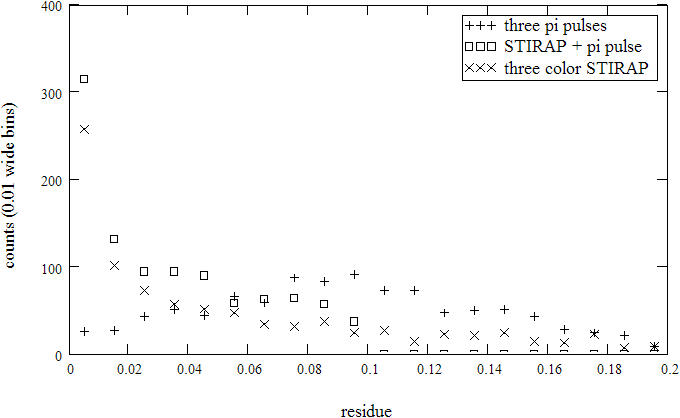
\includegraphics[width=5.00in]
{histogram/histogram.png}\\
\caption[Stochastic simulation histograms]{Stochastic simulation histograms. Notice that the three $\pi$ pulse sequence has a peak somewhere near 0.1 while the other two sequences seem peaked near zero.}
\label{histogram}
\end{figure} 
%----------------------------------------------------------------------------

%----------------------------------------------------------------------------
%----------------------------------------------------------------------------
%----------------------------------------------------------------------------
%----------------------------------------------------------------------------
%----------------------------------------------------------------------------
%----------------------------------------------------------------------------
